\section{Challenges}
\label{challenges:section}

Research on the algorithmic verification of quantum systems remains in its early stages.
%
Only recently have initial contributions emerged, including the first studies employing SAT solvers for quantum verification \citep{DBLP:conf/cade/ChenRT23}.
%
We have taken foundational steps in this direction through recent work on the symbolic verification of quantum circuits~\citep{PLanQC25,DBLP:journals/pacmpl/AbdullaCCHLLLT25,CACM25,ChenCLLTY23,ChenCLLT23,chen2025autoq}.
%
In contrast, the algorithmic verification of classical systems, particularly through model checking \citep{DBLP:reference/mc/AbdullaST18}, has been an active and well-established area of research for nearly four decades.
%
This field has yielded a substantial and mature body of work and continues to thrive, with ongoing research published regularly in premier venues such as {\sc POPL}, {\sc CAV}, {\sc PLDI}, {\sc MICRO}, {\sc ASPLOS}, etc.
%

While extending verification techniques to quantum systems is a natural and necessary progression, it also introduces a host of novel and technically challenging problems.
%
In the remainder of this section, we briefly review the current state of the art and its limitations.
%

\subsection{Symbolic Encodings}

Symbolic state space encodings have been among the most influential techniques in the verification of conventional programs over the past three decades.
%
By representing program semantics symbolically using various data structures and applying mathematical reasoning, one can efficiently verify whether a program satisfies its correctness properties.
%
These data structures encode logical formulas, allowing for both compact modeling of large or infinite state spaces and the efficient execution of logical operations.
%
Notable examples of symbolic representations that have significantly advanced the verification of classical systems include Binary Decision Diagrams (BDDs) for hardware verification and communication protocols, as well as automata over words and trees, for verifying parameterized systems and programs with dynamic heap structures.
%

Despite their success in conventional computing, the application of symbolic techniques remains limited in the quantum domain.
%
This limitation stems from quantum computation’s fundamentally different mathematical foundations, which involve state superposition, probabilistic measurement, and non-local entanglement—features that challenge conventional symbolic methods.
%
Nevertheless, with techniques likely to be developed in the future, symbolic verification will eventually play an equally important role in advancing the scalability and precision of quantum program verification.
%

As quantum computing continues to evolve, there is a growing need to develop symbolic abstractions tailored to quantum systems, hybrid symbolic-numeric approaches, and novel verification frameworks. These directions represent promising and largely unexplored areas of research.
%

In quantum circuit simulation, decision diagrams have been employed as compact representations of a single quantum state~\citep{TsaiJiangJhang2021,ChenChenJiangJobranovaLengal2024,KissingerWetering2022,10.1145/3712711}, and even of entire quantum circuits~\citep{WeiTsaiJhangJiang2022,SistlaChaudhuriReps2023,BurgholzerWille2020,Vinkhuijzen2023limdd}. While their application to verification against formal specifications remains underexplored, encoding entire quantum circuits as decision diagrams has potential for such verification tasks. Some efforts have also investigated leveraging constraint solvers for quantum circuit simulation and equivalence checking~\citep{MeiBonsangueLaarman2024Sim,MeiCoopmansLaarman2024Eq}.


Aside from a few notable exceptions~\citep{DBLP:journals/pacmpl/0001CLLTY23,DBLP:conf/fm/BauerMarquartLS23,Chareton2021,amy2018towards,fang2024symbolic} and our own recent contributions~\citep{PLanQC25,DBLP:journals/pacmpl/AbdullaCCHLLLT25,CACM25,ChenCLLTY23,ChenCLLT23,chen2025autoq}, there is a significant gap in research on symbolic encodings specifically designed for the automated verification of quantum circuits.
%
By contrast, several studies have focused on adapting classical Hoare logic to quantum systems. In particular, the approach proposed in \citep{d2006quantum} and Ying’s quantum Hoare logic \citep{ying2012floyd} defines predicates as mappings from mixed states—i.e., probability distributions over pure quantum states—to real values in the interval $[0,1]$, representing the probability that a given state satisfies a particular condition.
%
However, these logics are inherently deductive and interactive, not algorithmic in nature. As such, they are not suited for automated verification, often requiring significant manual effort and domain-specific reasoning.
%

An alternative is to adopt a fundamentally different approach by proposing a set-based methodology, where predicates are defined as mappings from quantum states to the Boolean domain $\{0,1\}$.
%
Within this framework, automata serve as compact representations of such predicates. A tree representing a quantum state is accepted by an automaton if and only if the corresponding predicate maps that state to 1.
%
One of the primary advantages of this set-based formulation is that it facilitates the construction of efficient and fully automated verification algorithms, making it significantly more scalable for practical use in the quantum domain.
%


Currently, there are no algorithms for minimization, simulation, and bisimulation over automata models designed specifically for the verification of quantum systems.
%
Addressing this gap should be a central objective.
%
We need to adapt and extend prior experience in classical automata theory to develop such algorithmic frameworks tailored to the specific characteristics of quantum systems.

\subsection{Algorithmic Verification}

%%%%%
\begin{figure}
\center
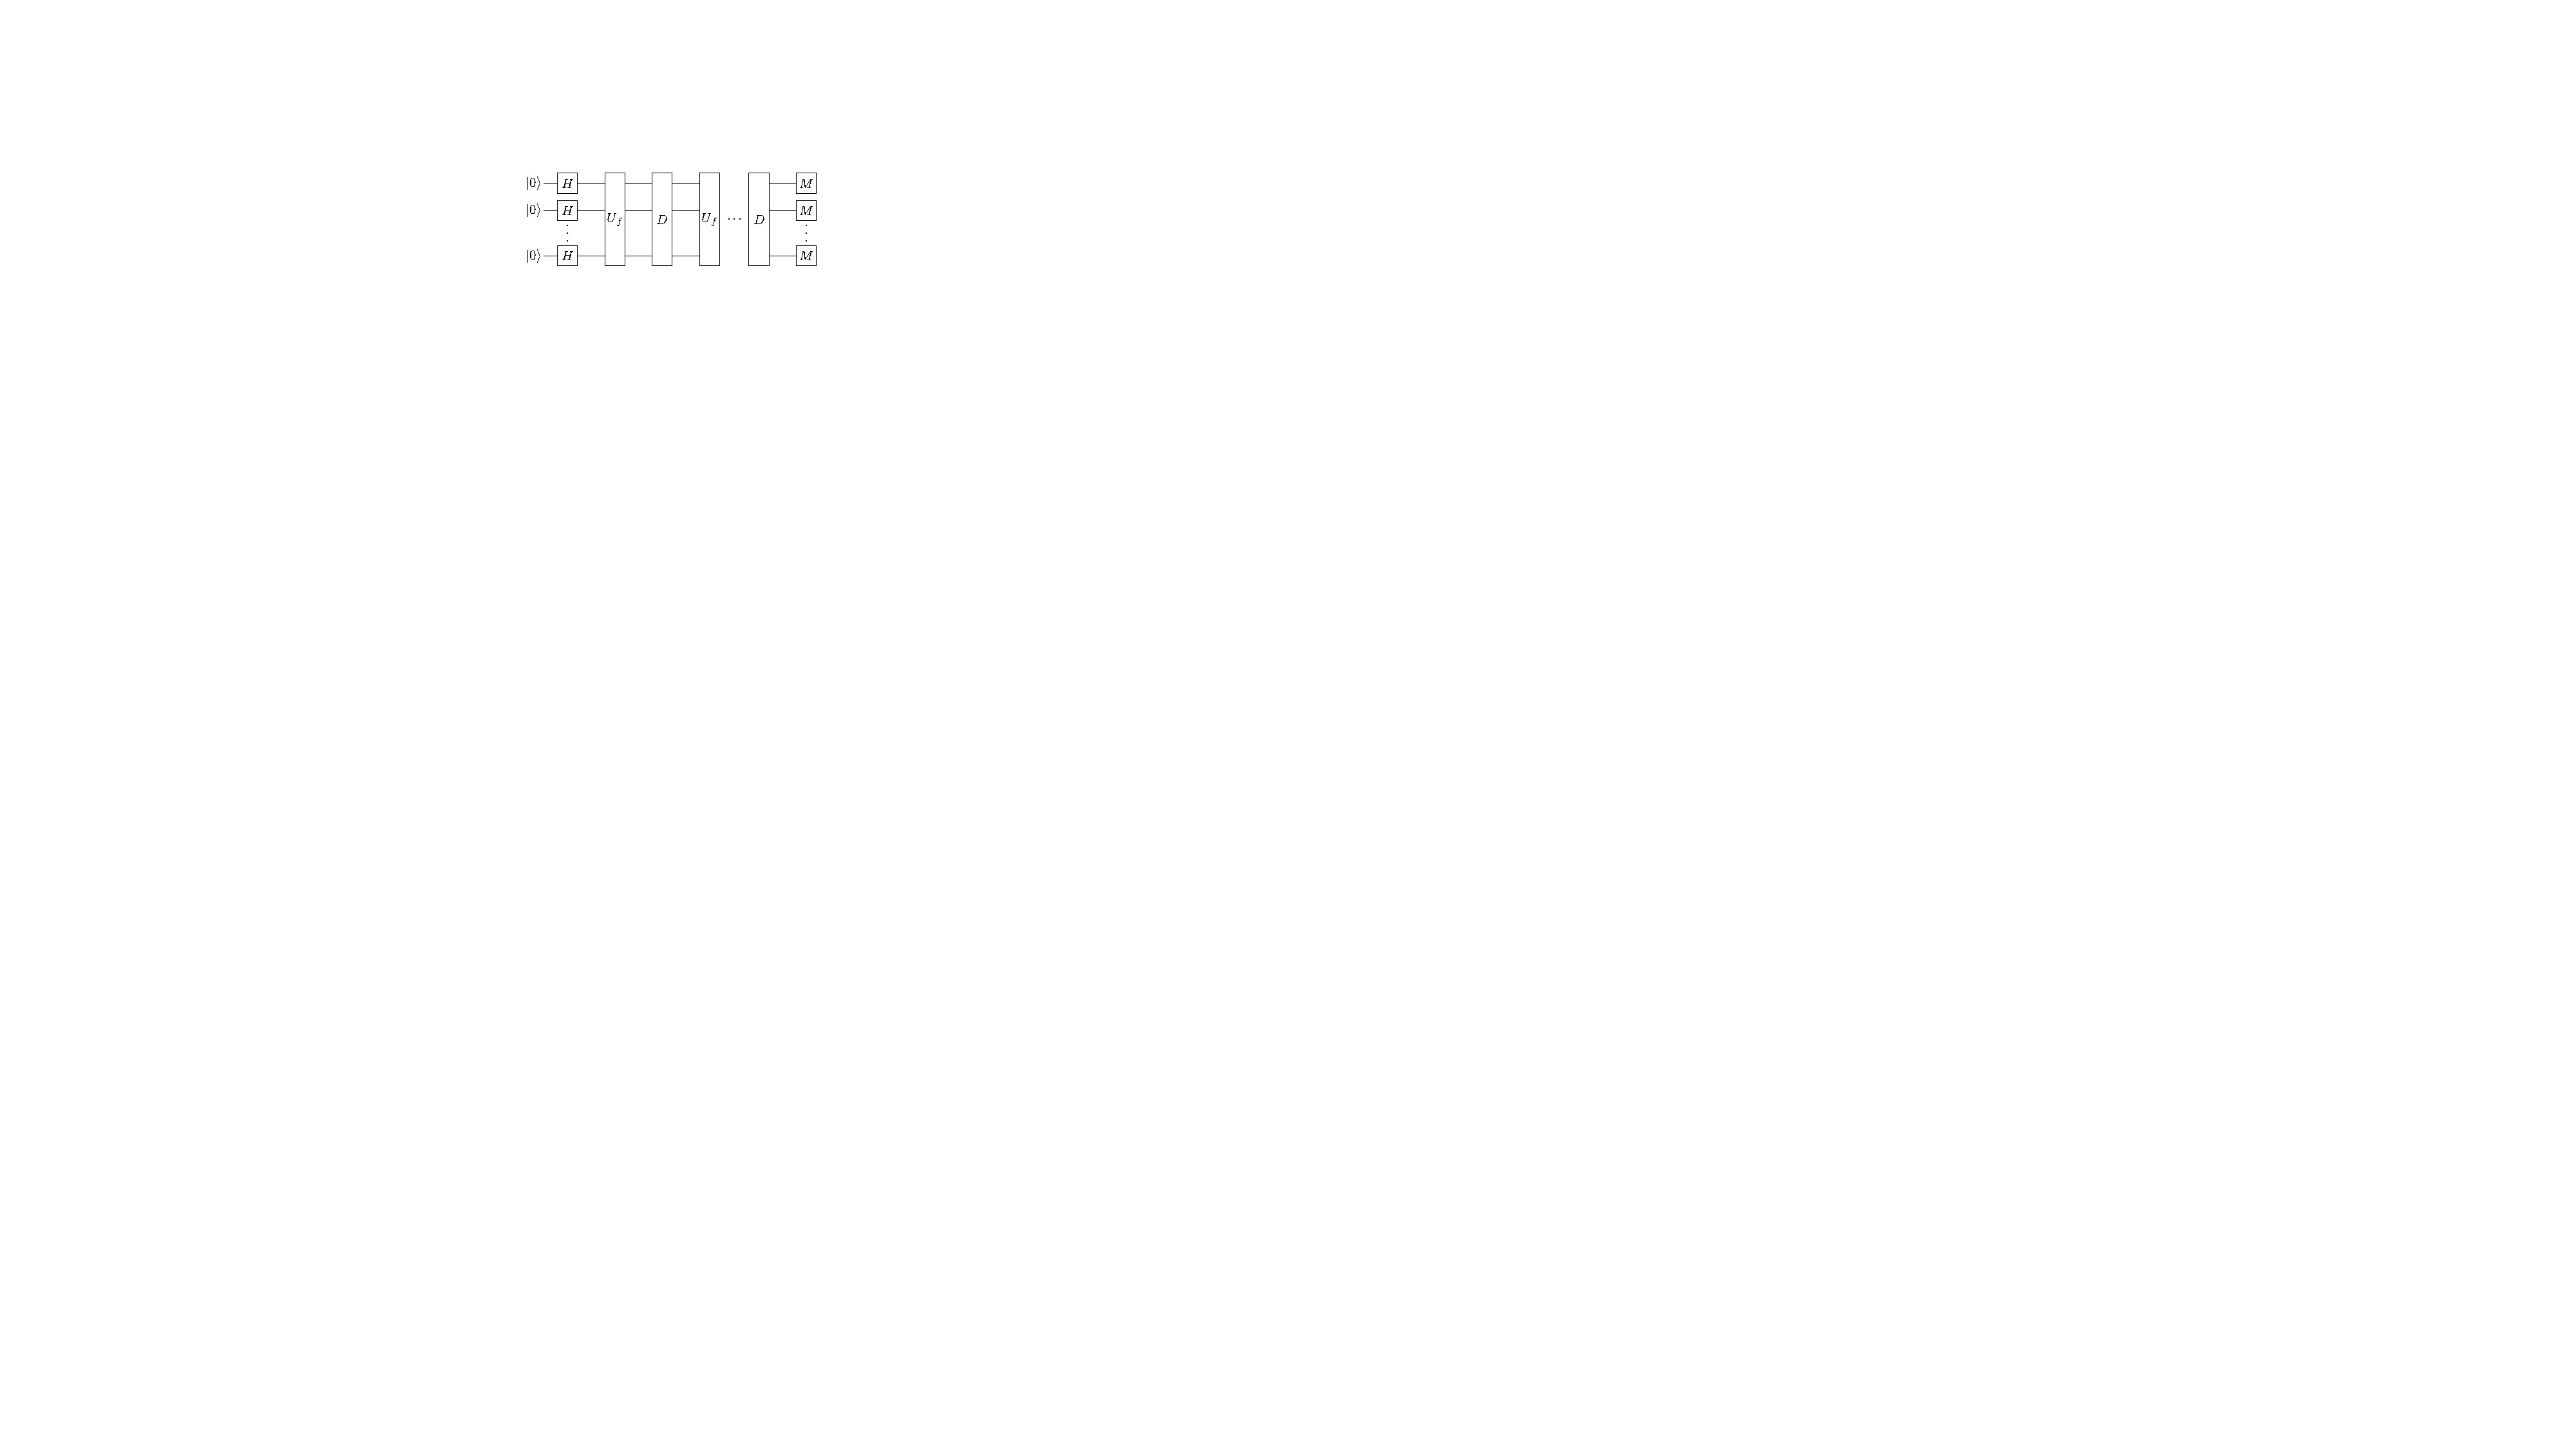
\includegraphics[scale=0.8]{Figures/Grover/Grover}
\caption{The classical Grover's search algorithm.}
\label{grover:fig}
\end{figure}
%

As previously mentioned, algorithmic verification techniques such as {\it model checking} have been among the most influential methodologies for checking the correctness of classical programs over the past three decades.
%
They offer an automated mechanism to determine whether a system satisfies a given specification.
%
Crucially, model checking is a complete verification method, meaning it can guarantee the absence of errors—unlike testing, which can only reveal the presence of bugs.
%
Nevertheless, extending model checking techniques to quantum systems presents considerable challenges due to three primary reasons.
%

First, as previously discussed, quantum systems involve state spaces of infinite size, even when the system comprises only a finite number of qubits.
%

Second, quantum systems are intrinsically parameterized, typically along two dimensions.
%
Consider, for instance, the circuit illustrated in \cref{grover:fig}, which implements the classical Grover’s algorithm.
%
This circuit accepts a Boolean function with $n$ input variables and aims to find an input for which the function evaluates to $1$.
%
If such an input exists, the circuit identifies one with a runtime of $O(\sqrt{N})$, where $N = 2^n$.
%
In contrast, any classical algorithm addressing the same problem would require $O(N)$ time.
%
Since the algorithm is constructed to operate on an arbitrary number of input qubits, there is no fixed upper bound on the input size.
%
Moreover, the system architecture comprises several stages, determined by $O(\sqrt{N})$.
%
Intuitively, each algorithm stage carries out one so-called {\it Grover rotation}.
%
This is an operation that increases the amplitudes of the basis states that satisfy the input function $f$.
%
By performing an increasing number of iterations, the precision of the computation increases, and the probability that we will measure the correct answer approaches one.
%
We reach the required precision after $O(\sqrt{N})$ iterations, which explains the number of stages\footnote{Again, we give a high-level description here. We refer, e.g., to \citep{10.5555/1408782} for the algorithm details.}.
%
The system is characterized by a two-dimensional parameterization: the number of qubits and the number of stages are unbounded.
%
We need to verify the system’s correctness across the entire space of possible values for these two parameters.
%

Third, unlike classical systems, quantum systems exhibit globally entangled transitions.
%
In general, the application of a gate to a single qubit may affect an exponential number of classical basis states. 
%
For instance, in \cref{qustate:tree:fig}, negating the qubit $x_1$ would swap the leaves in positions 1, 3, 5, and 7 with the leaves in positions 2, 4, 6, and 8, respectively.
%

The following aspects are currently lacking in existing work:
%
\begin{itemize}
\item
The paper \citep{BauerMarquartLS23} employs \emph{symbolic execution} \citep{10.1145/360248.360252} to verify input-output relationships by formulating queries discharged to SMT solvers over the theory of real numbers.
%
The SMT array theory approach \citep{DBLP:conf/cade/ChenRT23} instantiated this framework by enabling a polynomial-sized encoding of quantum circuits. Nevertheless, it continues to suffer from scalability limitations.
%
In \citep{DBLP:journals/pacmpl/AbdullaCCHLLLT25,PLanQC25}, we demonstrate that automata-based techniques outperform these approaches by several orders of magnitude.
%
Another scalable, fully automated method for analyzing quantum circuits is \emph{quantum abstract interpretation}~\citep{yu2021quantum,perdrix2008quantum}.
%
However, quantum abstract interpretation relies on over-approximation, which may limit its precision in bug detection.
%

\item
There are no methods supporting regular model checking or parameterized verification for quantum applications.
%
Our recent paper \citep{DBLP:journals/pacmpl/AbdullaCCHLLLT25} presents two examples of parameterized quantum circuits.
%
However, it does not provide algorithms for general parameterized verification.
%
We need to bridge this gap by designing and integrating model checking algorithms with abstraction techniques tailored for quantum systems.
\end{itemize}
